\chapter{Architecture}
\label{Architecture}
This chapter describes the software architecture of the product. It defines stakeholders, quality attributes, views, class diagram, patterns and tactics.
\newpage

\section{Stakeholders}

\subsection{Customer}
Our goal with this course was to create a product that not only works the way the customer intended, but does so with satisfactory performance. It also needed a clear, logical and functional architecture to make it easy to maintain. 
Our code needed to be written following the clean coding standard and make use of interfaces and general polymorphism, so that their developers could further develop this solution with ease.

\subsection{Implementers}
We wanted an architecture that would be easy to implement and would make sense to the coders of our own team as well as to those of the customer.

\subsection{Course Staff}
The course staff wants a clear and well-documented architecture that is easy to understand and evaluate.


\section{Quality Attributes}
The customer was very specific when it came to what they wanted when it came down to the product, they didn't specify any quality attributes but we could deduce the most common ones which we felt needed to be a part of the Quality attributes in our implementation, the following was deduced: Modifiability, Performance, Availability, Interoperability and Readability. 

\subsection{Modifiability}
While we were the create the solution for real estate ads specifically, the solution will be used for other ads as well. Therefore we need to make it modifiable so that other developers later on can further develop using our solution as a base.

\subsection{Performance}
We wanted the system to function with a satisfactory performance, even though the customer did not set any specific requirements for performance. For this reason, we decided to merely strive to achieve this goal by writing as efficient code as we could manage, making necessary changes to keep performance at a reasonable level. %TODO: Is this too vague?

\subsection{Availability}
The system should be available for the users when they need it. Therefore we needed to minimize the possible points of failure and the probability of these failing. %TODO: Too vague?

\subsection{Interoperability}
Our solution was only a part of the larger Webassistenten solution, and needed to inter-operate with already-existing order system. To achieve this goal, we used the same technology as requested by the customer, including Web API, MSSQL and so on.

\subsection{Readability}
The customer wanted us to write readable code. They requested that we used polymorphism by creating interfaces so that other developers can easily develop it further by developing plug-ins for the system. Readability is therefore important for easier further development of this system.


\section{Views}
Views are a way to display the implementation of a system by showing separate points of view associated with the various stakeholder concerns. We've tried to follow the 4+1 architectural view \footnote{\href{http://en.wikipedia.org/wiki/4+1_Architectural_View_Model}{http://en.wikipedia.org/wiki/4+1\_architectural\_view\_model}}
\subsection{Process view}
When we started out by designing the architecture we didn't know how the information flow was supposed to be and thereby didn't make a process view for the system. We also did not know how the internal system of Adressa works and how the processes in their system inter-operate. However we did create a new architecture to reflect on the changes we made during the project. 

\subsection{Logical view}
The logical view concerns the functionality the system provides by displaying it as a high level structure that shows how the components interact with each other. The logical view is usually a class diagram or sequence diagram. We've decided to use a class diagram because it's easier to see how the classes interact with each other and implement. Our logical view is based on the pattern Pipe and filter\footnote{\href{http://en.wikipedia.org/wiki/Pipeline_(software)}{http://en.wikipedia.org/wiki/Pipeline\_(software)}} due to the requirement of modifiability.
\begin{figure}[H]
\centering
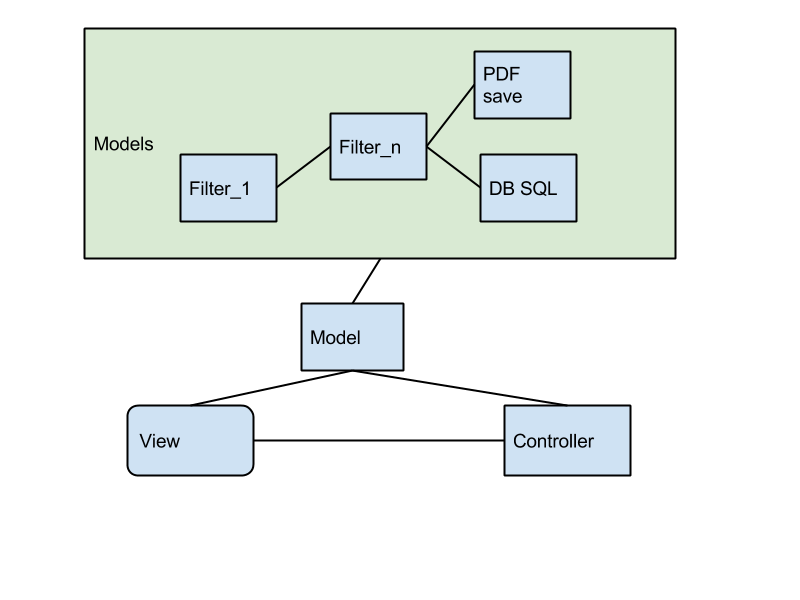
\includegraphics[width=0.8\textwidth]{images/architecture00.png}
\caption{Logical view}
\label{fig:logical_view}
\end{figure}


\subsection{Scenario view}
This view is also known as a use case view, which basically shows an example of an imagined and expected use of the system. The main purpose of this view is to show how the objects (in this case a client or a person) interacts with the processes and system.
\begin{figure}[H]
\centering
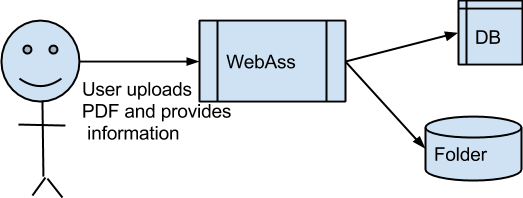
\includegraphics[width=0.8\textwidth]{images/architecture01.png}
\caption{Scenario view}
\label{fig:scenario_view}
\end{figure}




\subsection{Physical view}
The physical view shows how the physical components interacts with each other.
\begin{figure}[H]
\centering
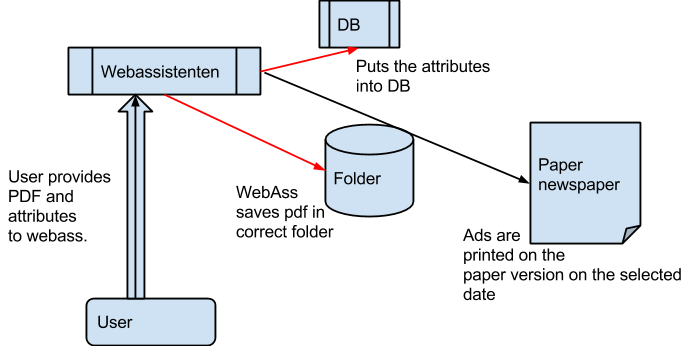
\includegraphics[width=0.8\textwidth]{images/architecture02.png}
\caption{Physical view}
\caption*{We are to implement the bold arrows}
\label{fig:physical_view}
\end{figure}
\newpage
\section{Class diagram}
From these views, we made this class diagram as a first draft of how we felt the system should be. However this later turned out to not fit into how the framework is supposed to be, and we had to change the architecture.
\begin{figure}[H]
\centering
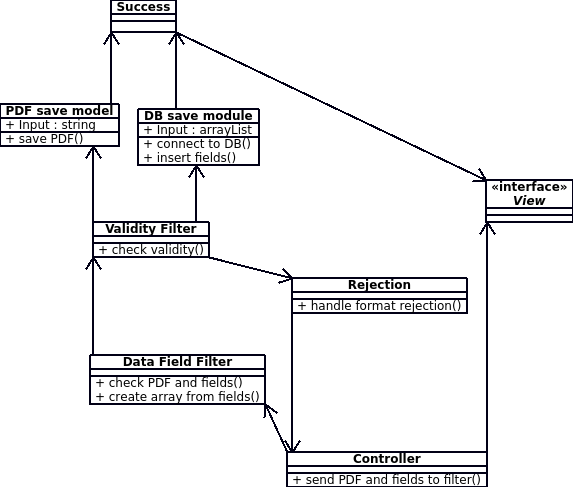
\includegraphics[width=0.8\textwidth]{diagrams/class_diagram.png}
\caption{Digital class diagram}
\label{fig:class_diagram}
\end{figure}
\section{Patterns}
Due to the project being a MVC.NET and Web API application we decided to use MVC pattern because the project might have this pattern built in already, we also wanted a pipe \& filter to filter the data and to satisfy the modifiability requirement.

\section{Tactics}
Architectural tactics are common strategies used to achieve the quality attributes required. These tactics should be kept in the back of ones head when developing this product.
\subsection{Modifiability}
\begin{itemize}
\item Increase semantic cohesion
\item Decrease coupling
\item Split modules
\end{itemize}

\subsection{Performance}
\begin{itemize}
\item Write optimal code
\end{itemize}

\subsection{Availability}
\begin{itemize}
\item Our code should not crash the customer's system, but it's their responsibility that the system is available.
\end{itemize}

\subsection{Interoperability}
\begin{itemize}
\item The technology and tools we're using should be sufficient to ensure interoperability.
\end{itemize}

\subsection{Readability}
\begin{itemize}
\item We will follow the clean coding principle and use camelCase coding and structure the code logically. The naming of classes and files should also be clear. Refer to \ref{Templates and Standards section} Templates and Standards section on page \pageref{Templates and Standards section}.
\end{itemize}

\section{Changes to the architecture}
When we started to implement the system we quickly found out that the we had architectural erosion because the architecture we designed in the start didn't fit well into the web api framework. After we got an overview of the system we had change the architecture to a MVC pattern. 
\begin{figure}[H]
\centering
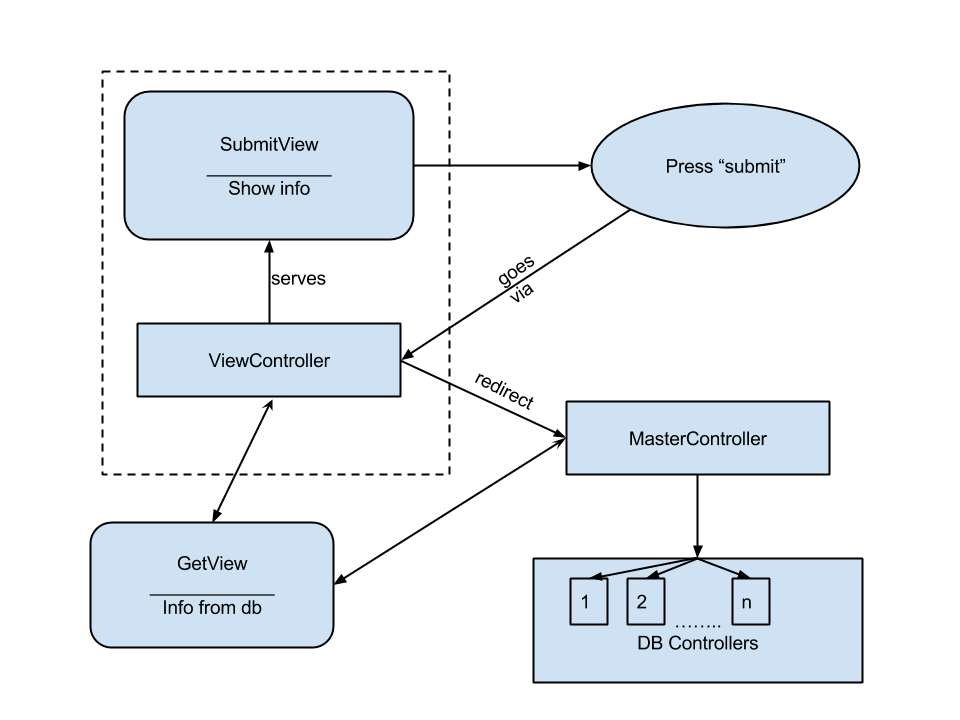
\includegraphics[width=0.8\textwidth]{images/architecture03_revised1.png}
\caption{Temporary process view}
\label{fig:info_flow}
\end{figure}
We tried to follow this MVC pattern when we implemented the system, however we quickly found out that the getView-Controller was not necessary.
\begin{center}
\begin{figure}[H]
\centering
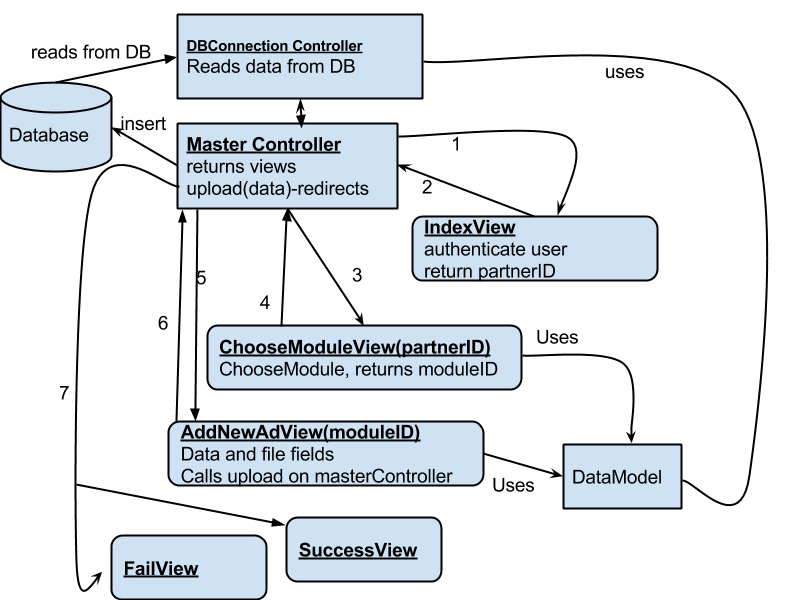
\includegraphics[width=0.9\textwidth]{images/architecture_final01.png}
\caption{Process View of Final Architecture}
\caption*{6 calls the upload method with files and data\\
7 is the upload method redirecting either to a FailView or a SuccessView}
\label{fig:process_view}
\end{figure}
\end{center}

\begin{center}
\begin{figure}[H]
\centering
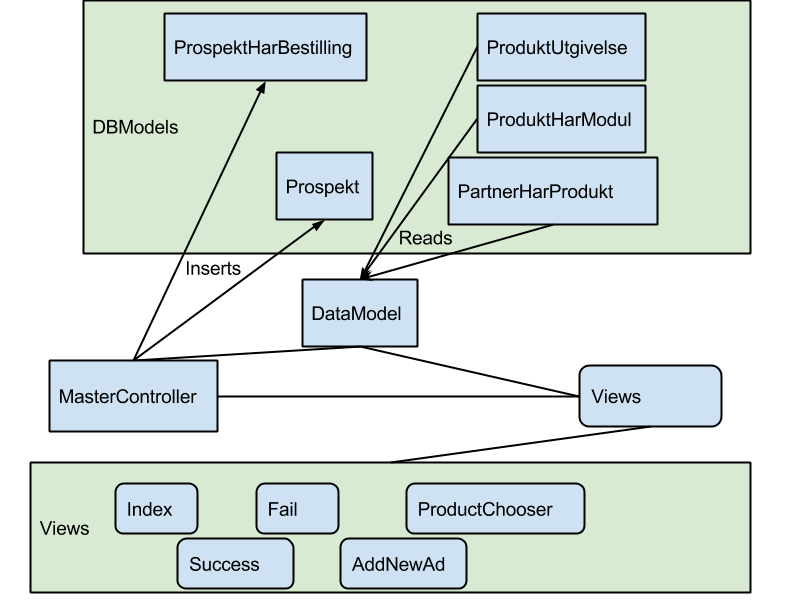
\includegraphics[width=0.9\textwidth]{images/architecture_final02.png}
\caption{Logical View of Final Architecture of MVC}
\caption*{This is the logical view of the MVC architecture.}
\label{fig:logical_view1}
\end{figure}
\end{center}


\begin{center}
\begin{figure}[H]
\centering
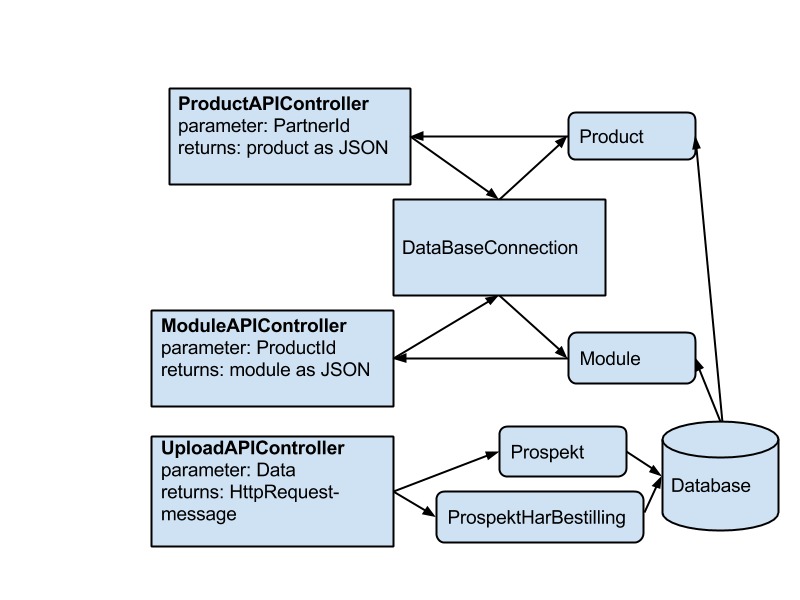
\includegraphics[width=0.9\textwidth]{images/architecture_finalwebapi01.png}
\caption{Logical View of Final Architecture of Web API}
%\caption*{This is the logical view of thearchitecture.}
\label{fig:process_view_webapi}
\end{figure}
\end{center}


